\chapter[Идентификация линейных стохастических систем второго типа]{%
  Идентификация линейных стохастических систем второго типа
}

\section{Математическая модель идентифицируемой системы}

Для обеспечения наглядности сравнения рассматривался случай
идентификации линейной скалярной системы.
В этом случае функция регрессии принимает простой вид:
\begin{equation}
  \psi = \alpha + \beta \xi,
  \label{eq:fun_linear_scalar}
\end{equation}
где \( \alpha, \beta \) "--- постоянная составляющая и коэффициент усиления "---
параметры системы. Модель задачи идентификации выглядит следующим образом:
\begin{equation}
  \label{eq:model_linear_scalar}
  \begin{aligned}
  h &= \alpha + \beta \xi, \\
  x &= \xi + \varepsilon_x, \\
  y &= h + \varepsilon_y,
  \end{aligned}
\end{equation}
где \( \xi, h \) "--- фактические значения входной и выходной переменной, \par
\( \alpha, \beta \) "--- фактические значения параметров объекта, \par
\( x, y \) "--- измеренные значения входной и выходной переменной, \par
\( \varepsilon_x, \varepsilon_y \) "--- независимые ошибки измерений значений входной и
выходной переменной, распределенные по нормальному закону:
\(
\varepsilon_x = N(0, \sigma_{\varepsilon_x}),
\varepsilon_y = N(0, \sigma_{\varepsilon_y})
\).

Данная модель использовалась для генерации наблюдений входа и выхода системы,
на основании которых были получены оценки её параметров методами на основе
классического и симметричного критериев аппроксимации.
Значения \( \xi_i \) выбирались из равномерного в \( [0, 10] \) распределения.
Для получения каждой оценки \( \hat{\alpha}, \hat{\beta} \) использовались результаты
ста наблюдений \( ( x_i, y_i ), i = \overline{1, n}, n = 100 \).

\section{Алгоритмы методов идентификации}

\subsection{Линейный метод наименьших квадратов}

Линейный метод наименьших квадратов ставит своей целью минимизировать сумму вертикальных расстояний
от аппроксимирующей гиперплоскости до результатов наблюдений.
Это соответствует использованию классического критерия идентификации:
\begin{equation*}
  \rho_{\text{к}} = \sum_i \rho_{\text{к}_i} \rightarrow \min.
\end{equation*}

Пусть \( y \) "--- вектор-столбец наблюдений выходной переменной \( \eta \),
а \( X \) "--- \( (r \times n) \)-матрица измерений вектора \( \xi \)
(\( r \) строк матрицы представляют собой векторы значений входных переменных в данном наблюдении,
а \( n \) столбцов "--- векторы значений данной входной переменной во всех наблюдениях).

Алгоритм получения МНК-оценок параметров линейной скалярно-векторной функции регрессии сводится
к вычислению значения вектора~\cite{wiki_lse}
\begin{equation*}
  \hat{\theta} = (X^{T}X)^{-1}X^{T} y.
\end{equation*}

Выполнение этого алгоритма требует времени, линейно зависящего от числа измерений \( O(n) \),
при выполнении реалистичного условия \( n \gg r \).

\vspace{2\baselineskip}
\subsection{Метод симметричной аппроксимации}

Метод симметричной аппроксимации минимизирует сумму перпендикулярных расстояний
от аппроксимирующей гиперплоскости до результатов наблюдений.
Это соответствует использованию симметричного критерия идентификации:
\begin{equation*}
  \rho_{\text{с}} = \sum_i \rho_{\text{с}_i} \rightarrow \min.
\end{equation*}

Пусть \( X \) "--- \( (m \times n) \)-матрица измерений.
Первые \( r \) и последние \( m - r \) строк этой матрицы представляют собой векторы наблюдений
входных и выходных переменных соответственно,
а столбцы соответствуют векторам \( X_i \) значений переменных в данном наблюдении.

Алгоритм расчета оценок параметров линейной функции регрессии
методом симметричной аппроксимации выглядит следующим образом~\cite{mukha_2016}:
\begin{enumerate}
\item Рассчитываются выборочные моменты случайного вектора наблюдений входных и выходных переменных:
  \begin{equation*}
    \hat{A} = \dfrac{1}{n} \sum_{i=1}^n X_i, \quad
    \hat{D} = \dfrac{1}{n}  \sum_{i=1}^n (X_i - A) (X_i - A)^T.
  \end{equation*}
\item Формируется матрица \( P \), состоящая из собственных векторов матрицы \( \hat{D} \),
  расположенных в порядке убывания соответствующих им собственных чисел.
\item Формируются матрица \( C \), состоящая из \( r \) первых столбцов матрицы
  \( P \). Выполняется разбиение матриц \( X \), \( \hat{A} \) и \( C \) на блоки:
  \begin{equation*}
    C =
    \begin{pmatrix}
      C_r \\
      C_{m-r}
    \end{pmatrix}, \quad
    X =
    \begin{pmatrix}
      X_r \\
      X_{m-r}
    \end{pmatrix}, \quad
    \hat{A} =
    \begin{pmatrix}
      \hat{A}_r \\
      \hat{A}_{m-r}
    \end{pmatrix}.
  \end{equation*}
  Таким образом, матрицы \( C_r \) и \( X_r \) содержат первые \( r \) строк матриц
  \( C \) и \( X \) соответственно,
  а \( C_{m-r} \) и \( X_{m-r} \) "--- последние \( m - r \) строк этих матриц.
  Вектор \( \hat{A}_r \) содержит первые \( r \),
  а \( \hat{A}_{m-r} \) "--- последние \( m - r \) элементов вектора \( \hat{A} \).
\item Рассчитываются значения оценок параметров зависимости~\eqref{eq:fun_linear_scalar}:
  \begin{equation*}
    \begin{aligned}
      \hat{\beta} &= C_{m-r} (C_r)^{-1}, \\
      \hat{\alpha} &= \hat{A}_{m-r} - \hat{\beta} \hat{A}_r.
    \end{aligned}
  \end{equation*}
\end{enumerate}

Подобно МНК, асимптотическая сложность этого алгоритма также составляет \( O(n) \),
считая \( n \gg m \).


\section{Численный анализ точности методов идентификации}

\subsection{Точность оценивания параметров}

Было выполнено сравнение точности оценивания параметров
\( \hat{\alpha}, \hat{\beta} \) системы~\eqref{eq:model_linear_scalar},
полученных классической линейной регрессией и методом симметричной аппроксимации,
в зависимости от c.~к.~о. ошибок наблюдений \( \sigma_{\varepsilon_x}, \sigma_{\varepsilon_y} \).

В качестве величины, характеризующей сравнительную точность оценивания параметров,
использовалась разность средних Евклидовых расстояний
между точными значениями параметров модели и их оценками,
полученными классической линейной регрессией и методом симметриченой аппроксимации:
\begin{equation}
  \begin{aligned}
    d &= d_{\text{к}} - d_{\text{с}}, \\
    d_{\text{к}} &= \frac{1}{k} \sum_{j=1}^k \sqrt{(\hat{\alpha}_{\text{к}_j} - \alpha)^2 + (\hat{\beta}_{\text{к}_j} - \beta)^2}, \\
    d_{\text{с}} &= \frac{1}{k} \sum_{j=1}^k \sqrt{(\hat{\alpha}_{\text{с}_j} - \alpha)^2 + (\hat{\beta}_{\text{с}_j} - \beta)^2}.
    \end{aligned}
  \label{eq:dst_linear_param}
\end{equation}

Расчеты величины \( d \) производились в узлах сетки значений
\( \sigma_{\varepsilon_x}, \sigma_{\varepsilon_y} \) в прямоугольнике
\( [0, 2] \times [0, 2] \) с шагом 0{,}1.
В каждом узле сетки вычислялось \( k = 100 \) оценок.

На рисунке~\ref{fig:comparison_linear_params_beta-small}
представлены графики зависимости величины~\eqref{eq:dst_linear_param}
от с.к.о. ошибок наблюдений \( \sigma_{\varepsilon_x}, \sigma_{\varepsilon_y} \) при
малых значениях коэффициента усиления модели \( \beta \).
Ввиду того, что при \( \sigma_{\varepsilon_y} > \sigma_{\varepsilon_x} \)
значение величины \( d \) невелико по модулю и отрицательно (\( d \in ( -0{,}5, 0 ] \)),
можно сделать вывод, что классическая линейная регрессия дает немного более точные оценки параметров,
чем метод симметриченой аппроксимации.
Поскольку при \( \sigma_{\varepsilon_y} \le \sigma_{\varepsilon_x} \) значение
\( d \) близко к нулю, можно утверждать, что точность оценок параметров,
полученных данными методами в приведенных условиях, одинакова.

\begin{figure}[p]
  \begin{subfigure}[b]{\linewidth}
    \centering
    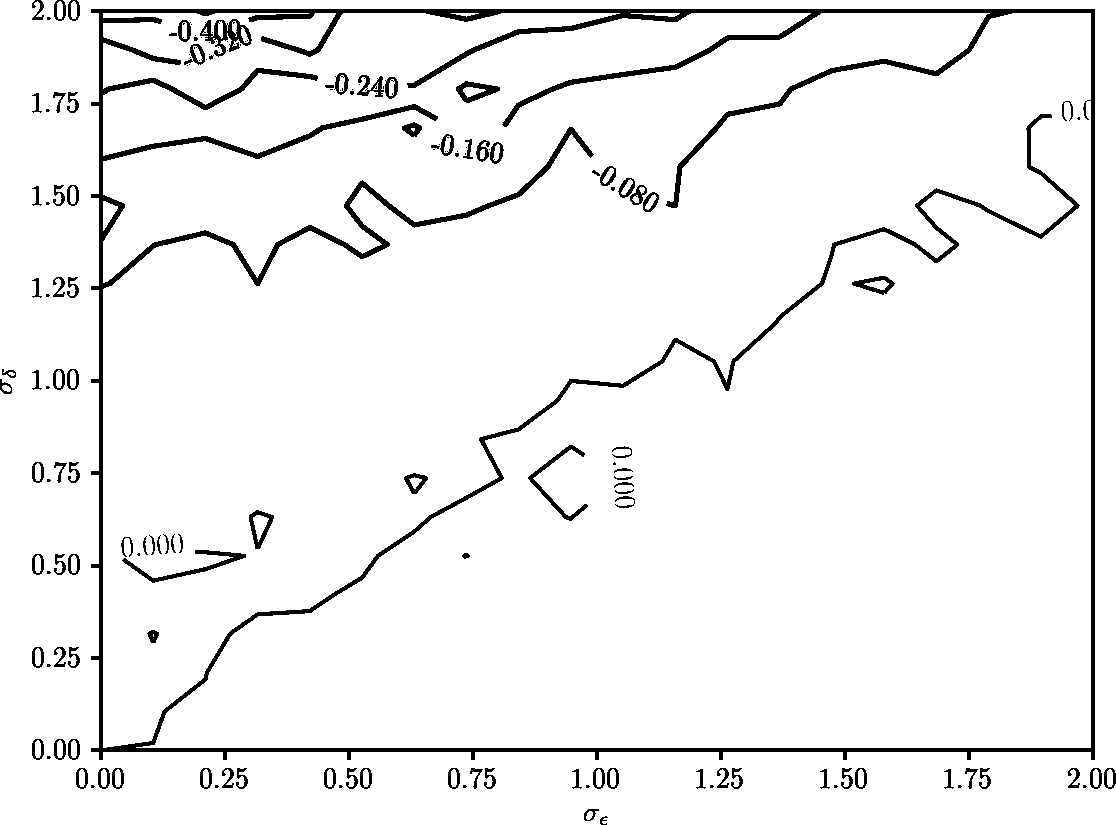
\includegraphics[width=135mm]{fig/linear/param/beta-0,125_param.png}
    \caption{\( \beta = 0{,}125 \)}
  \end{subfigure}

  \vspace{2\baselineskip}
  \begin{subfigure}[b]{\linewidth}
    \centering
    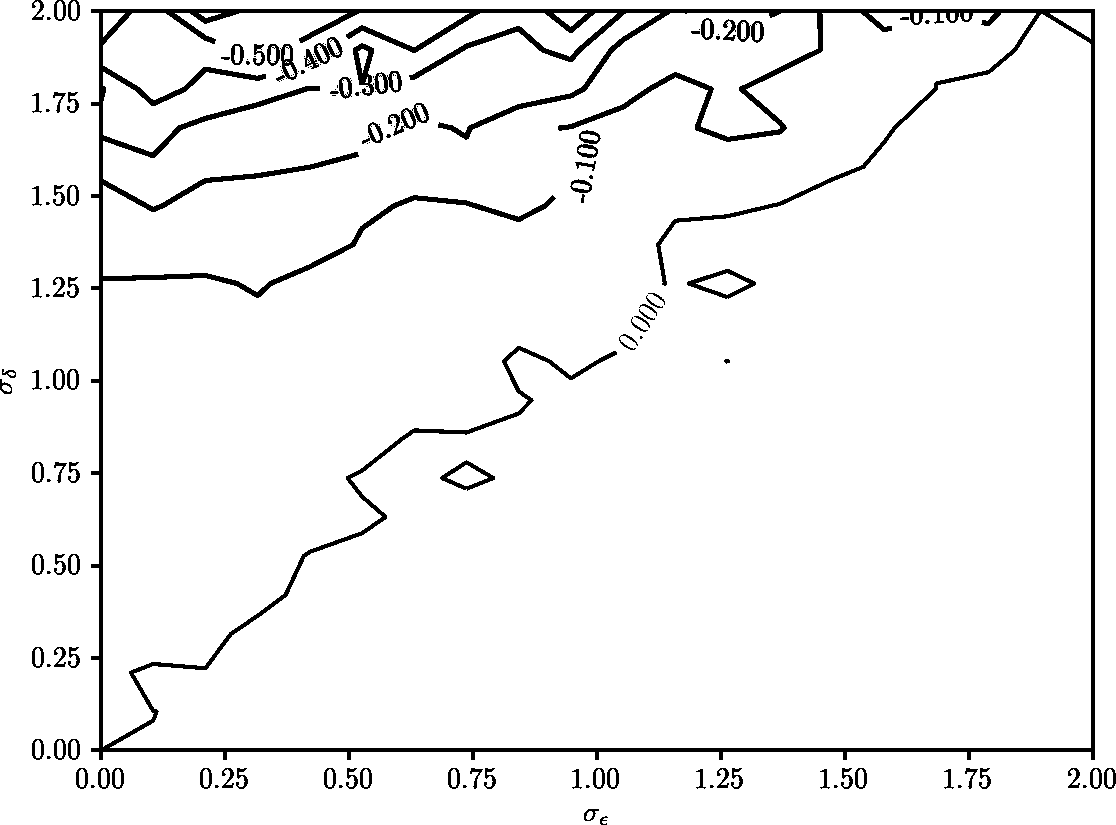
\includegraphics[width=135mm]{fig/linear/param/beta-0,2_param.png}
    \caption{\( \beta = 0{,}2 \)}
  \end{subfigure}

  \vspace{\baselineskip}
  \caption{%
    Точность оценивания параметров моделей с \\
    малыми коэффициентами усиления
  }\label{fig:comparison_linear_params_beta-small}
\end{figure}

На рисунке~\ref{fig:comparison_linear_params_beta-0,5}
представлен график функции \( d(\sigma_{\varepsilon_x}, \sigma_{\varepsilon_y}) \)
при \( \beta = 0{,}5 \).
Поскольку при \( \sigma_{\varepsilon_y} > \sigma_{\varepsilon_x} \)
значение \( d \) отрицательно (\( d \in ( -1, 0 ] \)),
классическая линейная регрессия дает более точные оценки параметров, чем МСА.
В отличие от предыдущего случая,
при \( \sigma_{\varepsilon_y} \le \sigma_{\varepsilon_x} \)
значение \( d \) положительно (\( d \in [0, 0{,}5 ) \)),
поэтому метод симметричной аппроксимации дает немного более точные оценки параметров,
чем классическая линейная регрессия.

\begin{figure}[t]
  \centering
  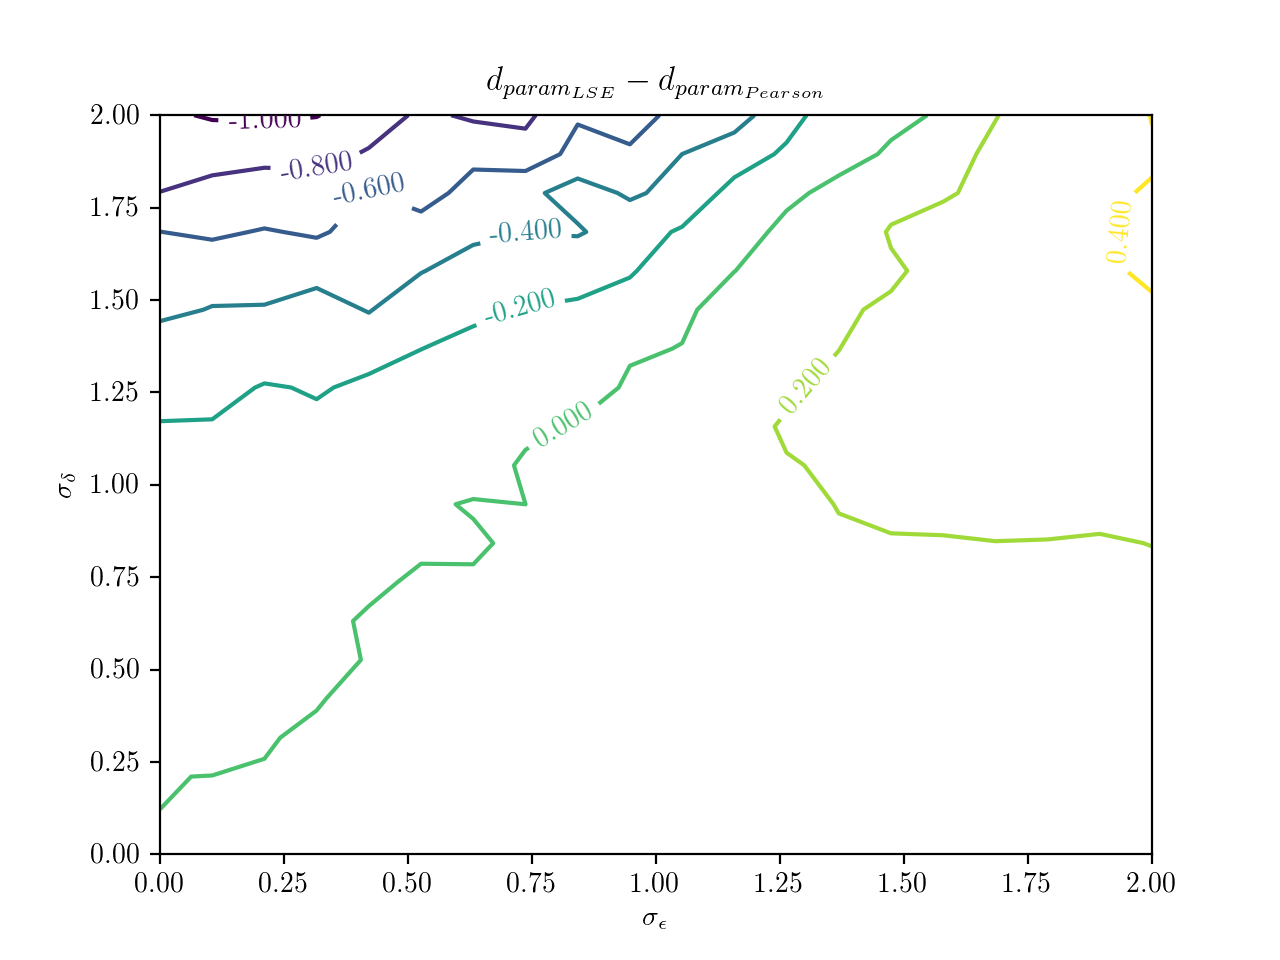
\includegraphics[width=135mm]{fig/linear/param/beta-0,5_param.png}
  \caption{%
    Точность оценивания параметров модели с \\
    коэффициентом усиления \( \beta = 0{,}5 \)
  }\label{fig:comparison_linear_params_beta-0,5}
\end{figure}

На рисунках~\ref{fig:comparison_linear_params_beta--1},~\ref{fig:comparison_linear_params_beta-1}
представлены графики функции \( d(\sigma_{\varepsilon_x}, \sigma_{\varepsilon_y}) \)
при \( \beta = -1 \) и \( \beta = 1 \) соответственно.
Поскольу эти графики практически совпадают, можно утверждать, что точность рассматриваемых
методов зависит от абсолютного значения коэффициента усиления \( \beta \) и не зависит от его знака.
Данное утверждение остается справедливым во всех рассмотренных случаях.

Красными точками отмечены пары значений с.~к.~о. ошибок наблюдений, при которых \( d = 0 \).
Эти значения были симметрично аппроксимированы линейными функциями,
представленными на графике прямыми красного цвета.
Прямые синего цвета соответствует приближенной зависимости~\eqref{eq:rule_linear_param}.

Нетрудно заметить, что на рассматриваемых графиках линии равного уровня функции
\( d(\sigma_{\varepsilon_x}, \sigma_{\varepsilon_y}) \)
симметричны относительно линии нулевого уровня данной функции.

При \( \sigma_{\varepsilon_y} > \sigma_{\varepsilon_x} \)
значение \( d \) отрицательно (\( d \in ( -1, 0 ] \)) ---
классическая линейная регрессия дает более точные оценки параметров, чем МСА.
При \( \sigma_{\varepsilon_y} \le \sigma_{\varepsilon_x} \)
значение \( d \) положительно (\( d \in [0, 1 ) \)),
поэтому метод симметричной аппроксимации дает более точные оценки параметров,
чем классическая линейная регрессия.

\begin{figure}[p]
  \begin{subfigure}[b]{\linewidth}
    \centering
    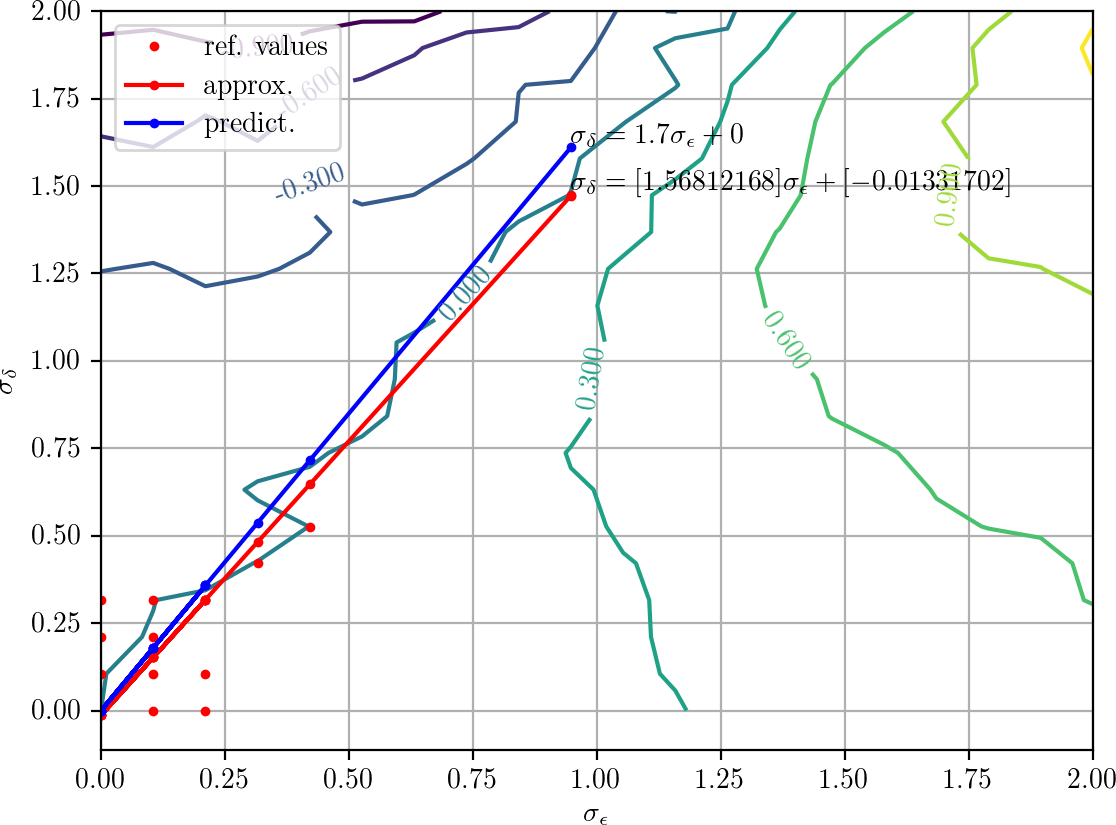
\includegraphics[width=135mm]{fig/linear/param/beta--1_param-accs-diff-approx}
    \caption{\( \beta = -1 \)}\label{fig:comparison_linear_params_beta--1}
  \end{subfigure}

  \vspace{2\baselineskip}
  \begin{subfigure}[b]{\linewidth}
    \centering
    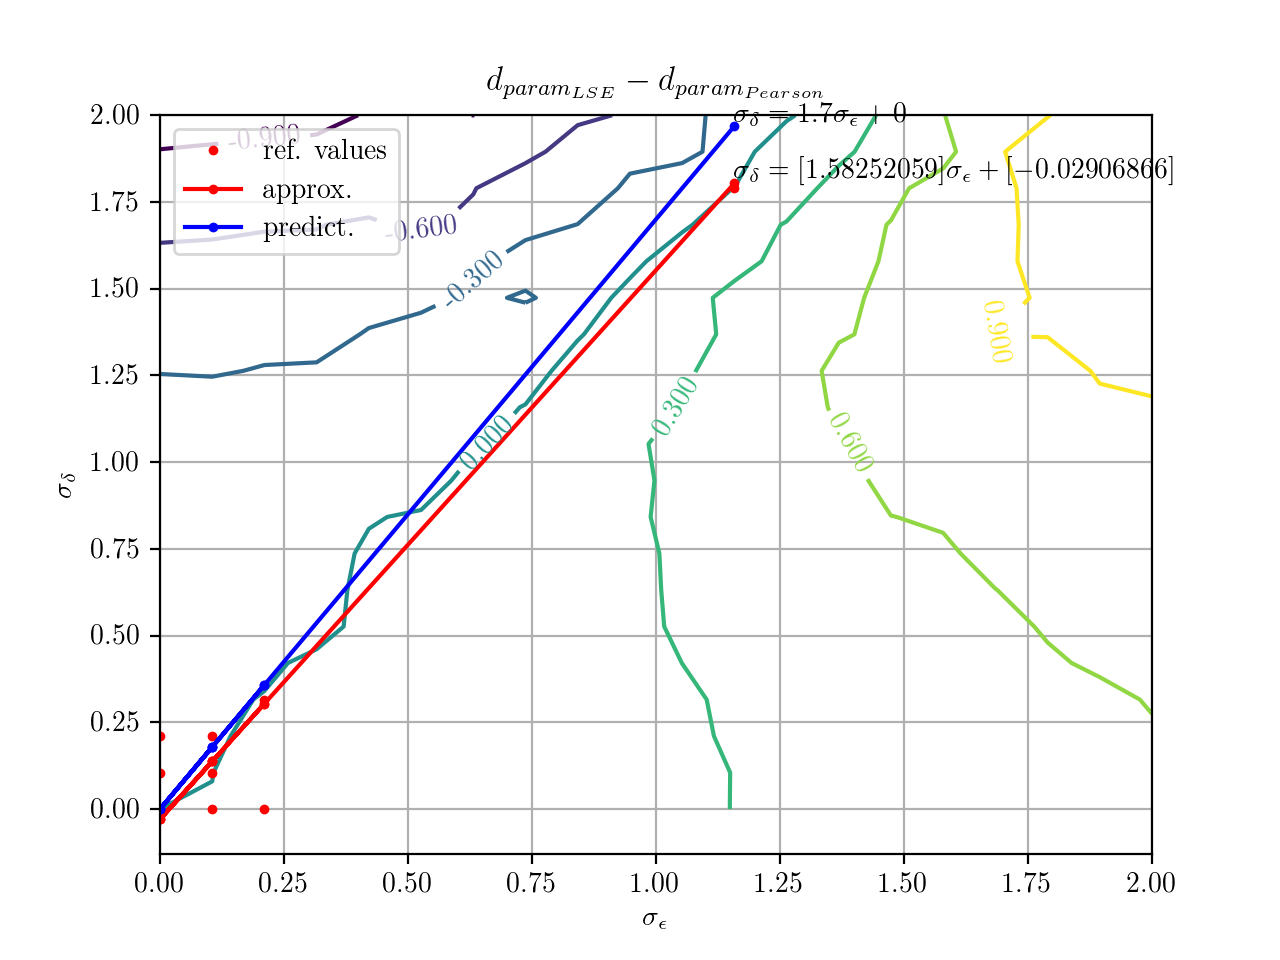
\includegraphics[width=135mm]{fig/linear/param/beta-1_param-accs-diff-approx}
    \caption{\( \beta = 1 \)}\label{fig:comparison_linear_params_beta-1}
  \end{subfigure}

  \vspace{\baselineskip}
  \caption{%
    Точность оценивания параметров моделей с \\
    единичным коэффициентом усиления
  }
\end{figure}

\newpage
На рисунке~\ref{fig:comparison_linear_params_beta-2}
представлен график функции \( d(\sigma_{\varepsilon_x}, \sigma_{\varepsilon_y}) \)
при \( \beta = 2 \).
Поскольку при \( \sigma_{\varepsilon_y} > 2 \sigma_{\varepsilon_x} \)
значение \( d \) невелико по модулю и отрицательно: \( d \in ( -0{,}5, 0 ] \),
классическая линейная регрессия дает более немного точные оценки параметров, чем МСА.
При \( \sigma_{\varepsilon_y} \le 2\sigma_{\varepsilon_x} \)
значение \( d \) положительно: \( d \in [0, 2{,}5 ) \),
поэтому МСА дает более точные оценки параметров,
чем классическая линейная регрессия.

\begin{figure}[h]
  \centering
  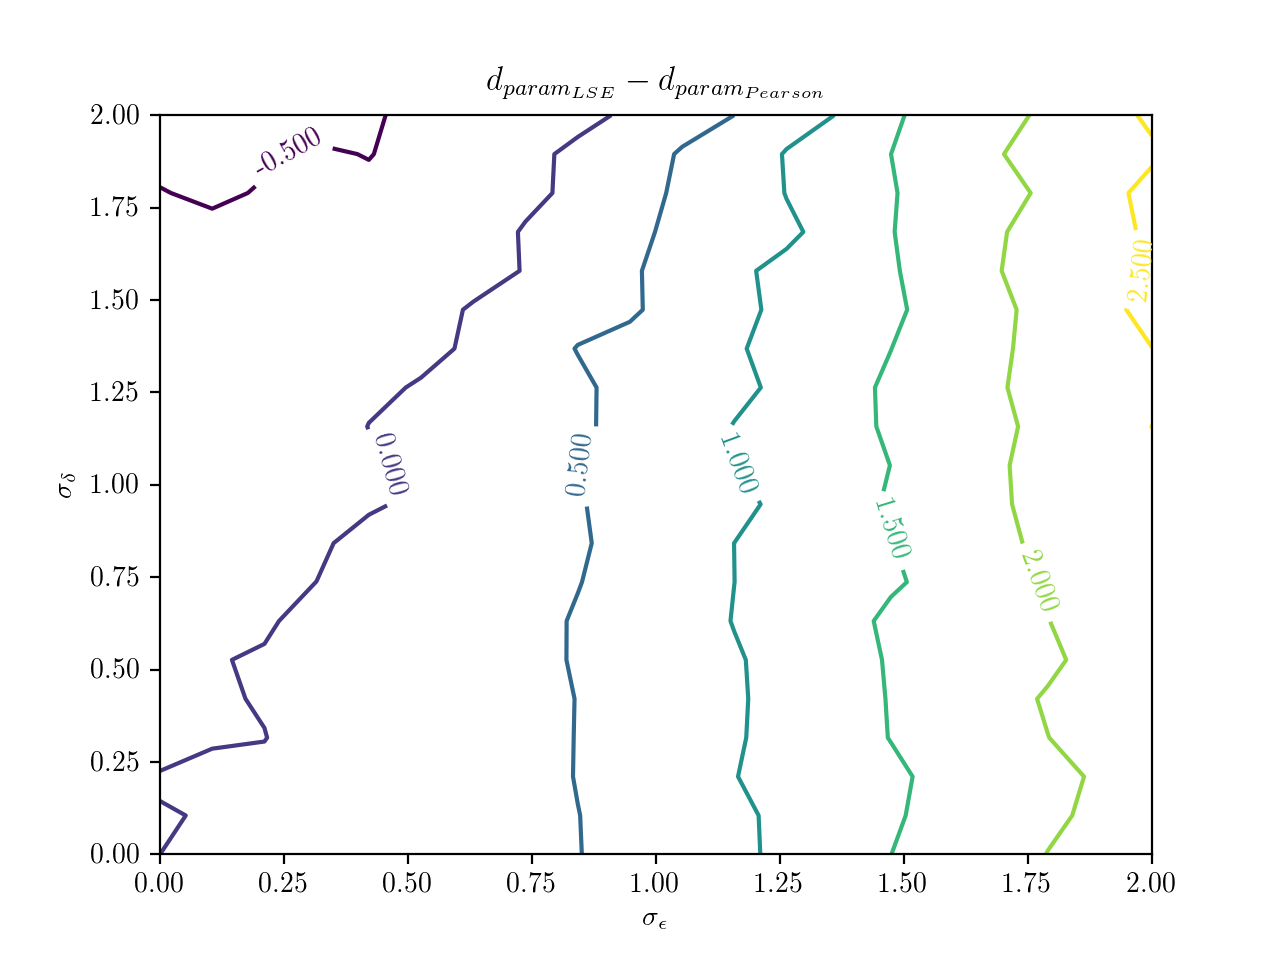
\includegraphics[width=135mm]{fig/linear/param/beta-2_param.png}
  \caption{%
    Точность оценивания параметров модели с \\
    коэффициентом усиления \( \beta = 2 \)
  }\label{fig:comparison_linear_params_beta-2}
\end{figure}

Следует отметить, что в рассмотренном случае область предпочтительного использования
МСА для оценивания точности параметров значительно больше,
чем у классической линейной регрессии,
а при \( \sigma_{\varepsilon_x} \gg \sigma_{\varepsilon_y} \) точность МСА значительно выше.

Данная тенденция усиливается при больших коэффициентах усиления модели
(рисунок~\ref{fig:comparison_linear_params_beta-big}).
При \( \sigma_{\varepsilon_y} > 8\sigma_{\varepsilon_x} \)
значение величины \( d \) невелико по модулю и отрицательно: \( d \in ( -0{,}5, 0 ] \),
классическая линейная регрессия дает немного более точные оценки параметров,
чем метод симметриченой аппроксимации.
При увеличении \( \sigma_{\varepsilon_y} \) относительно \( \sigma_{\varepsilon_x} \) значение
\( d \) быстро нарастает, что свидетельствует о том, что во-первых,
точность оценок параметров, полученных классической линейной регрессией при описанных условиях,
является посредственной,
а во-вторых, МСА дает значительно более точные оценки параметров,
чем классическая линейная регрессия.

\begin{figure}[p]
  \begin{subfigure}[b]{\linewidth}
    \centering
    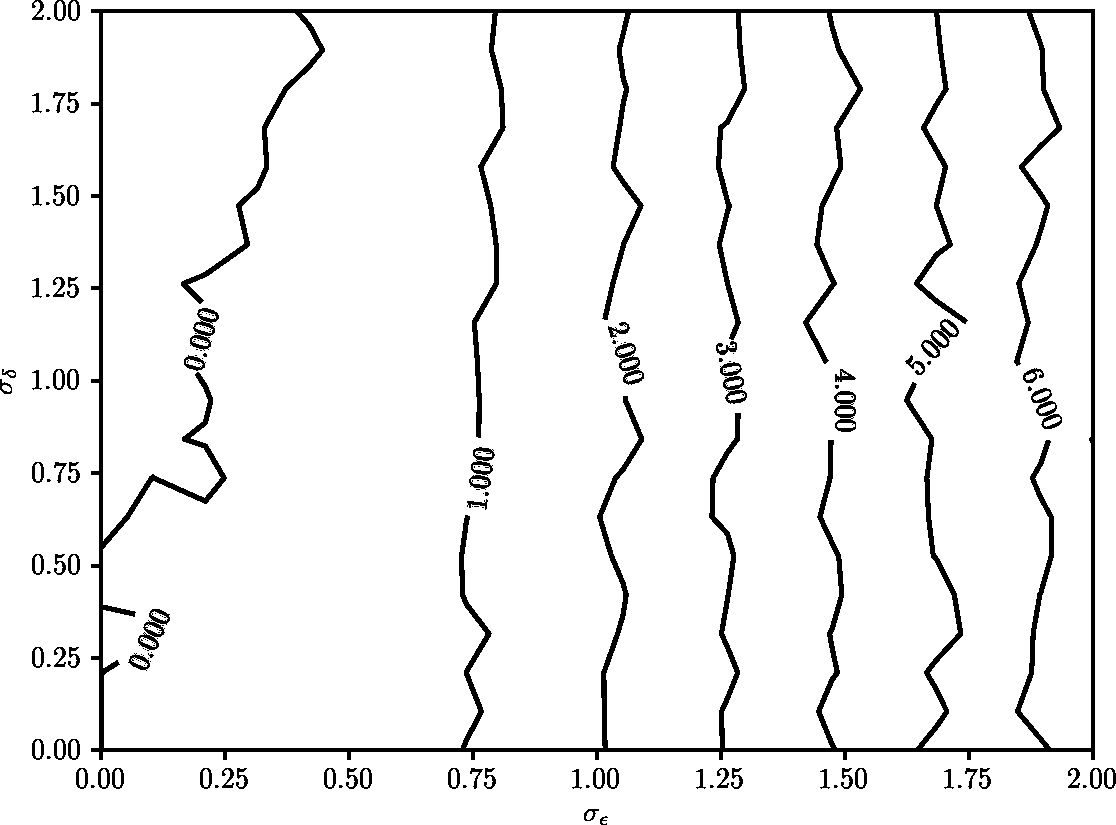
\includegraphics[width=135mm]{fig/linear/param/beta-5_param}
    \caption{\( \beta = 5 \)}
  \end{subfigure}

  \vspace{2\baselineskip}
  \begin{subfigure}[b]{\linewidth}
    \centering
    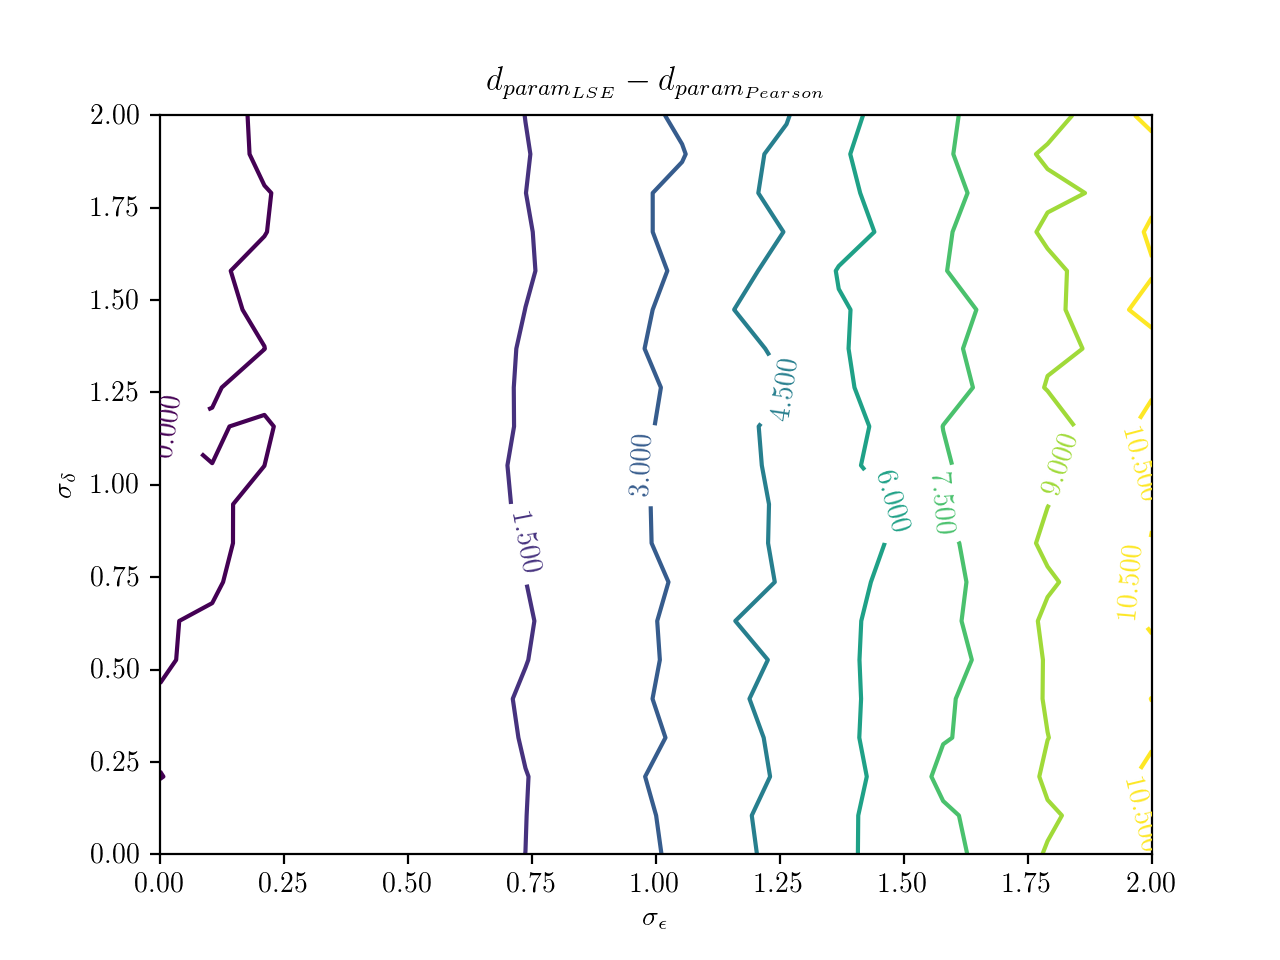
\includegraphics[width=135mm]{fig/linear/param/beta-8_param}
    \caption{\( \beta = 8 \)}
  \end{subfigure}

  \vspace{\baselineskip}
  \caption{%
    Точность оценивания параметров моделей с \\
    большими коэффициентами усиления
  }\label{fig:comparison_linear_params_beta-big}
\end{figure}

На основании изложенного можно сделать следуюшие выводы:
\begin{enumerate}
  \item Точность оценок параметров зависит от абсолютного значения коэффициента усиления системы и
    значений с.~к.~о. ошибок измерений входных и выходных переменных.
    С ростом величины коэффициента усиления и с.~к.~о. ошибок измерения
    метод симметричной аппроксимации дает более точные оценки,
    чем классическая линейная регрессия.
  \item При больших значениях коэффициента усиления \( |\beta| > 2 \)
    точность симметричного оценивания значительно превосходит
    точность классического подхода.
  \item Для того, чтобы решить, какой метод предпочтительно использовать для оценивания параметров
    линейной стохастической системы второго типа,
    предлагается использовать следующее эмпирическое правило:
    <<Если условие
    \begin{equation}
      \sigma_{\varepsilon_y} < (0{,}7 + |\beta|) \sigma_{\varepsilon_x}
      \label{eq:rule_linear_param}
    \end{equation}
    выполняется, то метод симметричной аппроксимации оценивает параметры системы
    второго типа более точно, чем классическая линейная регрессия>>.
\end{enumerate}

\newpage
\subsection{Точность прогнозирования наблюдений выхода}

Было выполнено сравнение точности прогнозирования наблюдений выхода по наблюдениям входа
системы~\eqref{eq:model_linear_scalar} со оценками параметров,
полученными классической линейной регрессией и методом симметричной аппроксимации,
в зависимости от c.~к.~о. ошибок наблюдений \( \sigma_{\varepsilon_x}, \sigma_{\varepsilon_y} \).

В качестве величины, характеризующей точность оценивания параметров,
использовалась разность средних Евклидовых расстояний в пространстве выходных наблюдений
между наблюдениями выхода модели и их оценками,
полученными классической линейной регрессией и методом симметриченой аппроксимации:
\begin{equation}
  \begin{aligned}
    d &= d_{\text{к}} - d_{\text{с}}, \\
    d_{\text{к}} &= \frac{1}{k} \sum_{j=1}^k \sqrt{ \sum_{i=1}^n (\hat{\alpha}_{\text{к}_j} + \hat{\beta}_{\text{к}_j} x_{ij} - y_{ij})^2}, \\
    d_{\text{с}} &= \frac{1}{k} \sum_{j=1}^k \sqrt{ \sum_{i=1}^n (\hat{\alpha}_{\text{с}_j} + \hat{\beta}_{\text{с}_j} x_{ij} - y_{ij})^2}.
    \end{aligned}
  \label{eq:dst_linear_predict}
\end{equation}

Расчеты расстояний~\eqref{eq:dst_linear_predict} производились в узлах сетки значений
\( \sigma_{\varepsilon_x}, \sigma_{\varepsilon_y} \) в прямоугольнике
\( [0, 2] \times [0, 2] \) с шагом 0{,}1.
В каждом узле сетки вычислялось \( k = 100 \) оценок.
Для получения каждой оценки \( \hat{\alpha}, \hat{\beta} \) использовались результаты
ста наблюдений \( ( x_i, y_i ), i = \overline{1, n}, n = 100 \).

На рисунке~\ref{fig:comparison_linear_predict} представлены графики зависимости
величины~\eqref{eq:dst_linear_predict},
от с.к.о. ошибок наблюдений \( \sigma_{\varepsilon_x}, \sigma_{\varepsilon_y} \) и
значений коэффициента усиления модели \( \beta \).
Нетрудно убедиться, что классическая линейная регрессия дает более точные оценки наблюдаений
выхода по наблюдениям входа системы, чем метод симметричной аппроксимации
во всем рассмотренном диапазоне значений коэффициента усиления и с.~к.~о. ошибок наблюдений.

\begin{figure}[h]
  \begin{subfigure}[b]{\linewidth}
    \centering
    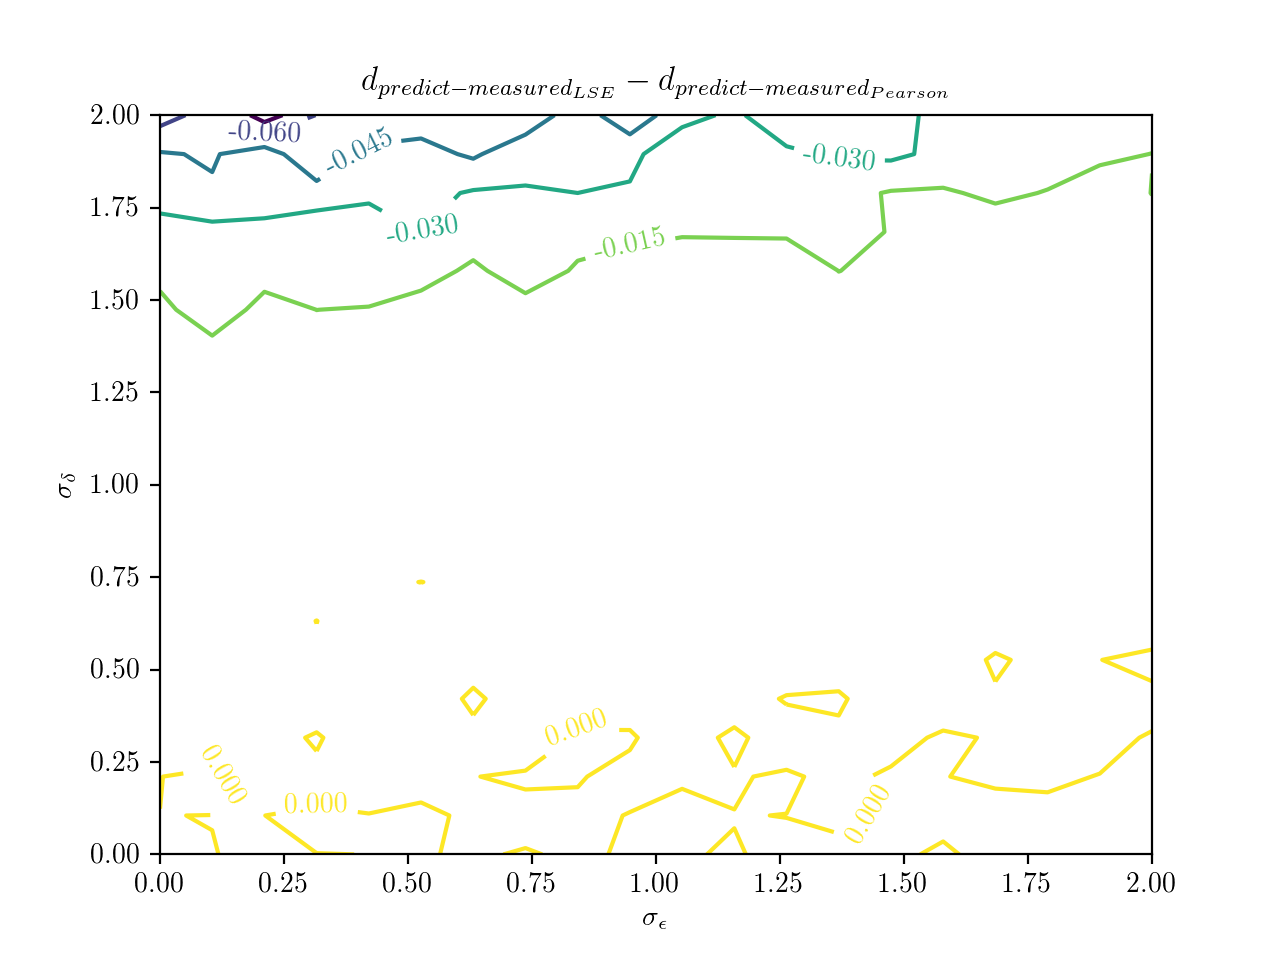
\includegraphics[width=135mm]{fig/linear/predict/beta-0,2_predict-measured.png}
    \caption{\( \beta = 0{,}2 \)}
  \end{subfigure}

  \vspace{2\baselineskip}
  \begin{subfigure}[b]{\linewidth}
    \centering
    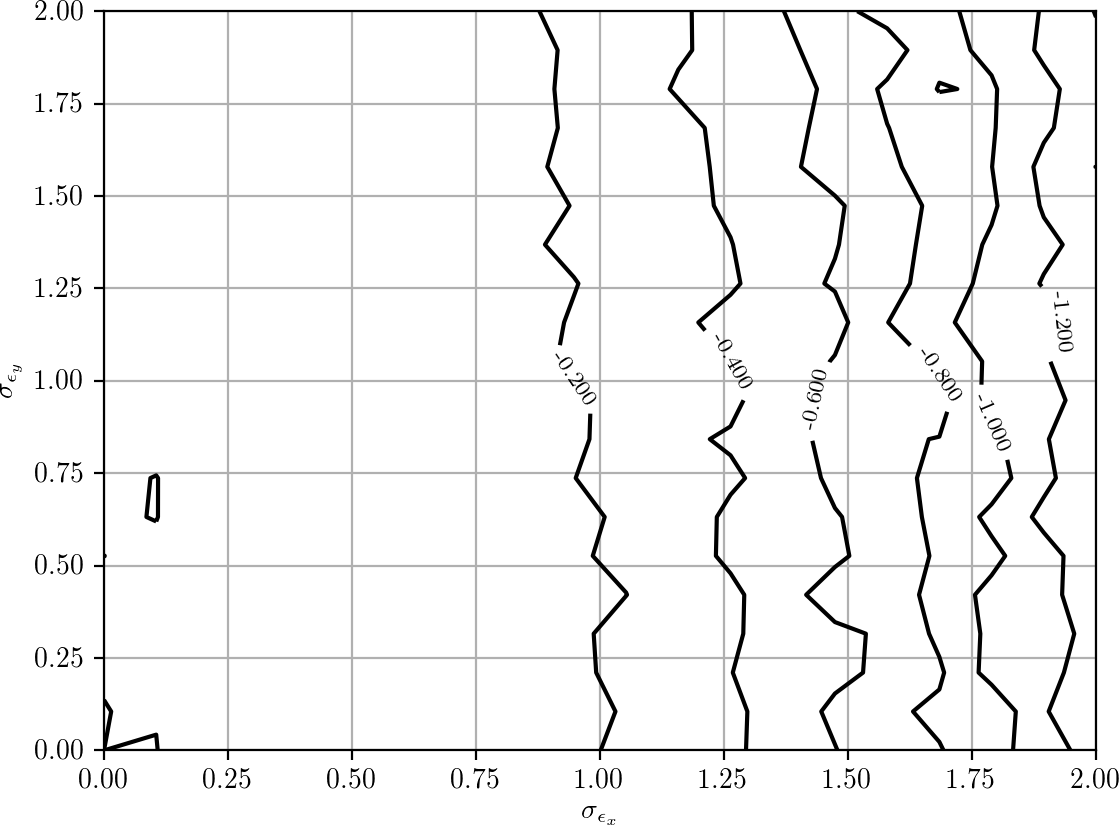
\includegraphics[width=135mm]{fig/linear/predict/beta-5_predict-measured.png}
    \caption{\( \beta = 5 \)}
  \end{subfigure}

  \vspace{\baselineskip}
  \caption{%
    Точность прогнозирования \\
    наблюдений выхода линейной модели
  }\label{fig:comparison_linear_predict}
\end{figure}
